%!TEX root = bambi-thesis.tex
\chapter{ROS} % (fold)
\label{appendix:ros}
\textit{"The Robot Operating System (ROS) is an opensource software framework supporting the development of complex, but modular systems in a distributed computing environment. While the core components of ROS are highly generic, the primary focus of ROS and its ecosystem is set to the development and research of robots. The performance critical parts of the framework are written in C++, but applications operating on top of the framework may currently be written in C++, Python or Lisp."}\cite{7795766} \par

\section{Concepts} % (fold)
\label{sec:concepts}
\begin{description}
    \item[Master] It provides name registration and lookup to the rest of the Computation Graph. Without the Master, nodes would not be able to find each other, exchange messages, or invoke services.
    \item[Nodes] are processes that perform computation. ROS is designed to be \textit{modular} at a fine-grained scale; a robot control system usually comprises many nodes. For example, one node controls a laser range-finder, one node controls the wheel motors, one node performs localization, one node performs path planning, one Node provides a graphical view of the system, and so on. A ROS node is written with the use of a ROS client library, such as roscpp or rospy
    \item[Parameter Server] It allows data to be stored by key in a central location. It is currently part of the Master.
    \item[Messages] Nodes communicate with each other by passing messages. A message is simply a data structure, comprising typed fields. Standard primitive types (integer, floating point, boolean, etc.) are supported, as are arrays of primitive types. Messages can include arbitrarily nested structures and arrays (much like C structs).
    \item[Topics] Messages are routed via a transport system with publish / subscribe semantics. A node sends out a message by publishing it to a given topic. The topic is a name that is used to identify the content of the message. A node that is interested in a certain kind of data will subscribe to the appropriate topic. There may be multiple concurrent publishers and subscribers for a single topic, and a single node may publish and/or subscribe to multiple topics. In general, publishers and subscribers are not aware of each others’ existence. The idea is to decouple the production of information from its consumption. Logically, one can think of a topic as a strongly typed message bus. Each bus has a name, and anyone can connect to the bus to send or receive messages as long as they are the right type.
    \item[Services] The publish / subscribe model is a very flexible communication paradigm, but its many-to-many, one-way transport is not appropriate for request / reply interactions, which are often required in a distributed system. Request / reply is done via services, which are defined by a pair of message structures: one for the request and one for the reply. A providing node offers a service under a name and a client uses the service by sending the request message and awaiting the reply. ROS client libraries generally present this interaction to the programmer as if it were a remote procedure call.
    \item[Bags]A format for saving and playing back ROS message data. Bags are an important mechanism for storing data, such as sensor data, that can be difficult to collect but is necessary for developing and testing algorithms.
\end{description}
\begin{figure}[ht]
    \centering
    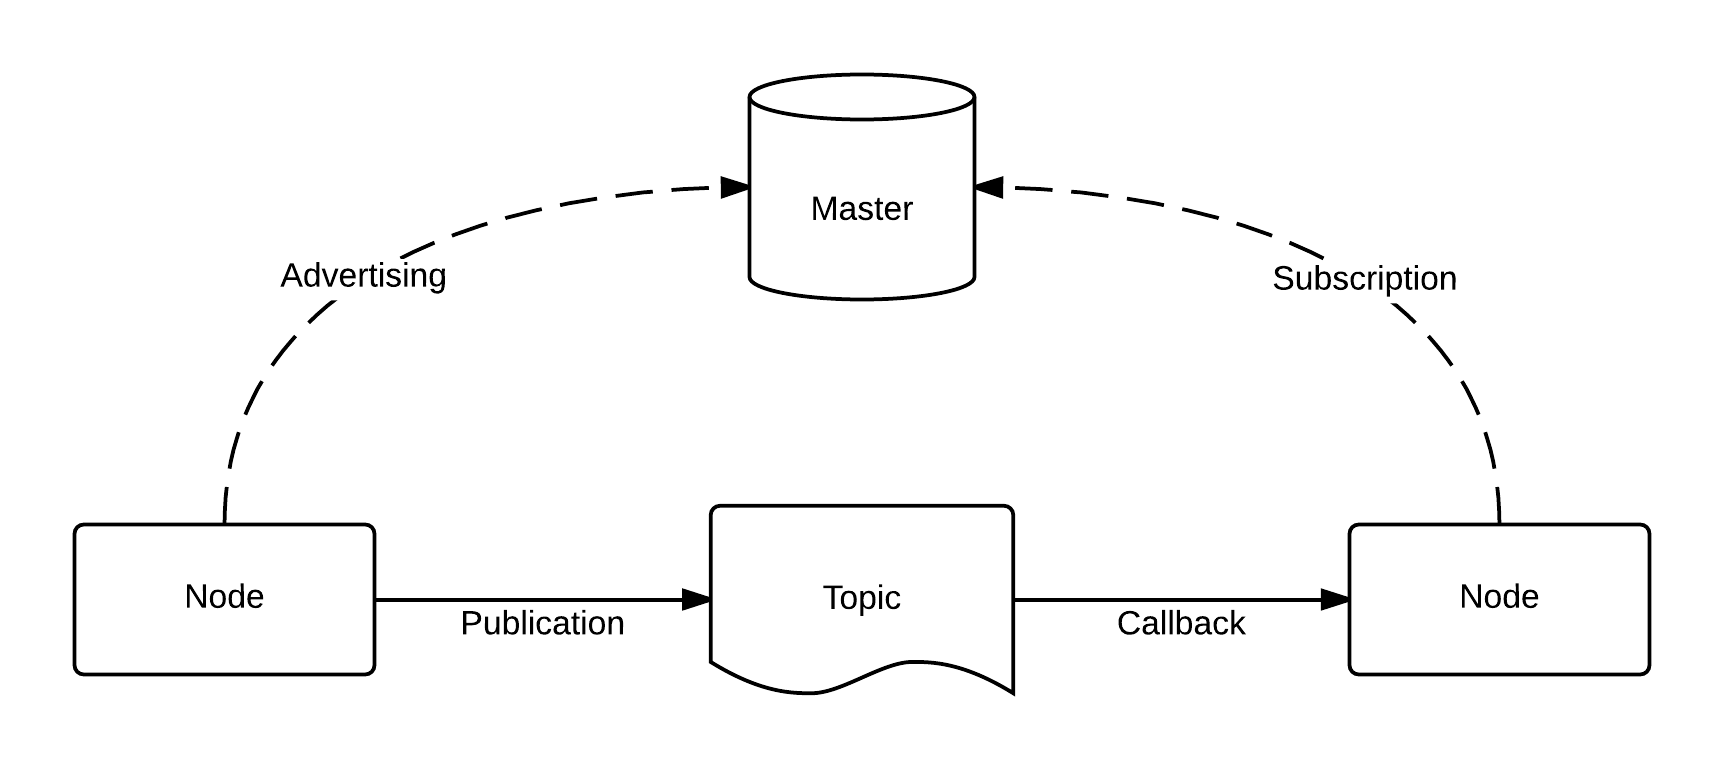
\includegraphics[width=1\textwidth]{figures/A1/ROS-master-node-topic.png}
    \caption{ROS Nodes communication}
    \label{fig:ROS-architecture}
\end{figure}
% section concepts (end)
% chapter ros (end)